\documentclass[10pt]{extarticle}

\usepackage{extsizes}
\usepackage{listings}
\usepackage{amsmath}
\usepackage{xcolor}
\usepackage{enumerate}
\usepackage[margin=1in]{geometry}
\usepackage{subfiles}
\usepackage{graphicx}
\usepackage{wrapfig}
\usepackage[binary-units=true]{siunitx}
\usepackage{subfig}
\usepackage{caption}
% \usepackage{hyperref}


\lstset{
basicstyle=\ttfamily,
numbers=none,
numberstyle=\small,
tabsize=4,
columns=flexible,
showstringspaces=false,
showtabs=false,
keepspaces,
captionpos=b,
escapeinside={<@}{@>}
}

\title{Garbage Collection on Lox}
\author{Tobias Pristupin}
\date{June, 2021}

\begin{document}

\title{\vspace{-2.0cm}
\includegraphics[scale=0.1]{washu_logo.png} 
\\[1cm]
Garbage Collection on Lox}
\maketitle
\tableofcontents
% \newpage

\section{Project Overview}
This project was a semester long effort under the guidance and mentorship of Professor Jonathan Shidal from the Computer Science department at Washington University in St. Louis.

\medskip
The goal of this independent research project was twofold. First, develop a compiler and VM from scratch for the Lox programming language. Second, implement different Garbage Collection (GC) algorithms for the Lox compiler, and benchmark them using Lox programs. 

The first section of this paper introduces the Lox language and gives an overview of the compiler's implementation. The second section discusses the two GC algorithms implemented in the Lox compiler, followed by a series of benchmarks comparing their performance and effectiveness in varying scenarios.

\medskip
All the code for this project can be found at https://github.com/TobiPristupin/lox-compiler.

\section{The Lox Language and Compiler}
The Lox language was created by Bob Nystrom in his book "Crafting Interpreters". The book documents the process for developing an Abstract Syntax Tree (AST) interpreter in Java and a compiler with a stack based VM in C, both for the Lox language. This research project is based around the compiler. 

The compiler for this project was written in C++ instead of C, in order to take advantage of modern features such as standard support for OOP, RAII, smart pointers, etc. A main objective of the compiler's development was to write it in native and idiomatic C++, instead of simply "porting" the book's C implementation to C++.

\subsection{What is Lox}

Lox is a dynamically typed language with support for OOP. It's syntax is a mixture of C's traditional syntax with Python's dynamically typed syntax. It has all the features a modern language should have, such as functions, scope, classes, inheritance, closures, lambdas, and support for a standard library \footnote{Since the focus of this project was on garbage collection, some of these features were omitted from the compiler. A previous implementation of an AST interpreter for Lox, that supports every language feature  (and some extra features that the book does not include), can be found at www.pristu.dev}. Here is an example program:

\begin{lstlisting}
    fun fib(n){
        if (n == 1 || n == 2){
            return 1;
        }
        return fib(n-1) + fib(n-2)
    }

    var result = fib(5);
    print result;

    class Shape {
        init(sides){
            this.sides = sides;
        }
    }

    class Square < Shape {
        init(color){
            super.init(4);
            this.color = color;
        }
    }

    var square = Square("red");
\end{lstlisting}

\subsection{The Lox Compiler}

The Lox compiler is a bytecode compiler, that also includes a stack based VM for that bytecode. This allows the compiler to run in any platform. For example, the following Lox program: 

\begin{lstlisting}
    var x = 10;
    if (x <= 10) {
        print true;
    }
\end{lstlisting}
Compiles to the following set of bytecode instructions:
\begin{lstlisting}
    OP_CONSTANT x
    OP_CONSTANT 10
    OP_DEFINE_GLOBAL x
    OP_CONSTANT x
    OP_GET_GLOBAL x
    OP_CONSTANT 10
    OP_GREATER
    OP_NOT
    OP_JUMP_IF_FALSE 6
    OP_POP
    OP_TRUE
    OP_PRINT
    OP_JUMP 1
    OP_POP
    OP_RETURN
\end{lstlisting}
Which are then executed by the VM to produce the output \lstinline{true}.

\section{Garbage Collection on Lox}

The second objective of the project was to implement various garbage collection algorithms for the Lox compiler, and benchmark them in different scenarios. Two GC algorithms were implemented in this project: \textbf{Mark Sweep} and \textbf{Reference Counting}.

\subsection{Mark Sweep}

As the name suggests, Mark Sweep can be divided into two phases: 

\begin{enumerate}
    \item \textbf{Mark Phase:} This phase involves distinguishing live objects from garbage. Every object that is reachable by the running program will be marked as such. This is accomplished by running a Depth-First Search (DFS) traversal starting from a root set of immediate references (objects currently on the stack, global and static variables) and recursively visiting every inner reference of those objects. 

    \item \textbf{Sweep Phase:} The sweep phase involves \textit{sweeping} all the objects that are garbage. Since every reachable object has been already marked as such by the mark phase, this phase only involves iterating through all objects in the heap and deleting those that haven't been marked.
    
\end{enumerate}

Under the hood, the Lox compiler keeps track of all objects currently in the heap using a linked list. Every object has a boolean flag representing if it was marked or not. 

\medskip
A major concern for Mark Sweep is deciding when to run a GC cycle. This concern is amplified by the fact that the implementation for the Lox compiler is stop-the-world, which means that all program execution must be halted while the garbage collector runs \footnote{An alternative to this would be a concurrent garbage collector, which runs in a separate thread from the main program and can perform garbage collection as the program runs.}. Every GC cycle requires all program execution to halt, so we aim to minimize the number of cycles. However, by minimizing cycles, the time it takes for an individual cycle to complete increases, since more garbage objects accumulate in the heap in between cycles. Deciding on a frequency for the GC is a delicate balancing act between how many interruptions a running program will have, and how long those interruptions will be.

The Lox compiler solves this problem in a simple but elegant way: keep track of the amount of bytes currently allocated by the program. Once that amount exceeds a determined threshold, trigger a garbage collection cycle (causing the number of allocated bytes to decrease). After the cycle is completed, update the threshold for the next cycle using the following formula: \[\text{threshold} = \text{\# of allocated bytes} * 2\]This ensures that the threshold changes dynamically, accommodating the memory requirements of the program at that point in time.

\subsection{Reference Counting}

Reference counting is based on the following idea: count the number of pointer references to each allocated object. When an object has no references pointing to it, it is inaccessible and can be safely deleted. When an object is deleted, any objects referenced by that object get their respective  reference counts (refcounts) decremented by one. 

A main advantage of Reference Counting over Mark Sweep is that objects are deleted as soon as they reach a refcount of zero and can no longer be referenced, instead of having to wait for the next GC cycle. Deleting objects incrementally ensures that GC overhead is distributed across the program, resulting in a smoother and more responsive system when compared to tracing collectors such as Mark Sweep.

However, Reference Counting has two big disadvantages. First of all, significant overhead can be incurred when updating reference counts. Sometimes thousands of updates are performed on a single object before reaching a count of zero. Second, Reference Counting has no mechanism to reclaim cyclic storage. Any object which refers directly or indirectly to itself, such as a node in a doubly linked list, will never be deleted by a Reference Counting collector. This is because that object will never reach a refcount of zero, even if it is inaccessible by the rest of the program.

\subsection{Benchmarking and Comparison}

\subsubsection{The \lstinline{collect and allocate} keywords}

To facilitate benchmarking, two special keywords were added to the Lox language.

\begin{enumerate}
    \item The \lstinline{allocate} expression: Provides an easy way to allocate a chunk of memory in the heap. The expression \lstinline{allocate x} will return a reference to a chunk of memory of size \lstinline{x} kilobytes. Behind the scenes, this is implemented in the compiler as \lstinline{new char[x * 1024]}.
    \item The \lstinline{collect} statement: When using Mark Sweep, it can be hard to determine exactly when a cycle will be triggered. \lstinline{collect} will force a GC cycle,  regardless of the current threshold and state of the program. This keyword has no effect when used under Reference Counting. 
\end{enumerate}

\subsubsection{Cycles Benchmark}

Cycles are a major weakness of Reference Counting. Most Reference Counting implementations have no efficient way of dealing with them. The following Lox program simulates a scenario with cycles.

\begin{lstlisting}[numbers=left]
    class Node {}

    var head = Node();
    head.next = Node();
    head.next.next = Node();
    head.next.next.next = head;

    head = nil;

    collect;
\end{lstlisting}

This program creates a cycle of length three. In line 8, the only reference to the head node is cleared, rendering the cycle inaccessible by the rest of the program and thus garbage. Line 10 forces a garbage collection when using Mark Sweep.

\medskip
Compiling the program and running it with the VM generates logging output regarding memory usage and garbage collection. This data is then manipulated using a Python script and converted into a graph describing the program's memory usage. These are the graphs generated when using Mark Sweep and Reference Counting as our choice of GC algorithm:

\newpage

\begin{figure}[h]%
    \centering
    \subfloat[\centering Mark Sweep]{{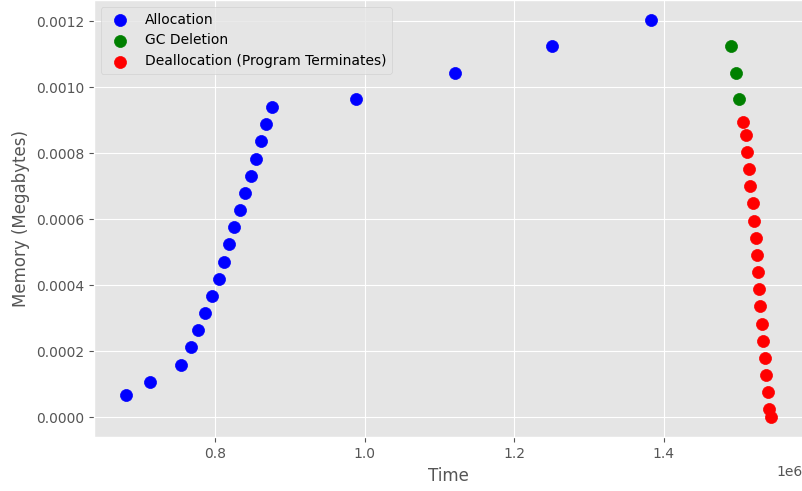
\includegraphics[width=0.47\textwidth]{marksweep_cycles.png}}}%
    \qquad
    \subfloat[\centering Reference Counting]{{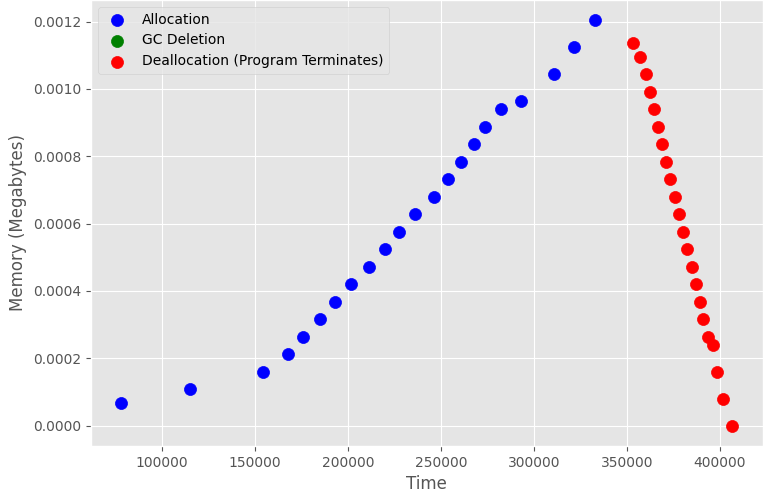
\includegraphics[width=0.47\textwidth]{refcounting_cycles.png} }}%
    \caption{Memory usage for cycles benchmark}
\end{figure}

The blue circles represent memory allocated. The green circles represent memory deleted by the GC. The red circles represent the memory deleted once the program terminates (not deleted by the GC). The graph on the left has three green dots, showing that when using a Mark Sweep collector, the three nodes created by the program were promptly deleted. On the other hand, on the right we can observe how there are no green dots, only blue and red. This is because the Reference Counting collector failed to recognize the three nodes in the linked list as garbage, since they form a cycle and their refcounts will never reach zero. 

\medskip
There are multiple ways to handle cycles with Reference Counting, but all of them involve some tradeoff regarding performance or complexity. The most common approach is to allow cycles to be created, and run a tracing garbage collector such as Mark Sweep periodically to delete all cycles. Another approach is to introduce the use of \textit{strong} and \textit{weak} references. Weak references are just like strong references, but they cannot keep an object alive on their own. This is the solution employed by shared pointers in C++.

\subsubsection{Large Heap Benchmark}

A major problem with Mark Sweep is that the cost of each collection cycle is proportional to the size of the heap. All live objects must be visited and marked in each cycle, and all garbage objects must be deleted in the sweep phase. This imposes a fundamental limitation in the efficiency of the algorithm. The following Lox program explores this.

\begin{lstlisting}[numbers=left]
    class Node {}

    var head = Node();
    head.memory = allocate 1;

    var current = head;
    for (var i = 0; i < 1000; i = i + 1){
        current.next = Node();
        current = current.next;
        current.memory = allocate 1;
    }

    var x = allocate 1;
    for (var i = 0; i < 200; i = i + 1){
        x = allocate 1;
        collect;
    }
\end{lstlisting}

This program first creates a linked list of size 1000. Each node has a \lstinline{memory} field, that contains a chunk of memory of \SI{1}{\kilo\byte}. The variable \lstinline{head} contains a reference to this list. \lstinline{head} is never cleared, so the list always remains a live object. After that, 200 chunks of \SI{1}{\kilo\byte} are allocated in the heap. Note that the variable \lstinline{x} is always overwritten, so after every iteration the previously allocated memory chunk becomes unreachable and thus garbage. Line 16 forces a garbage collection cycle after every iteration (when using Mark Sweep). The purpose of this program is to stress Mark Sweep by simulating a scenario where GC cycles are constantly triggered when there are many live objects in the heap. 

\medskip
Running the program using Mark Sweep and Reference Counting generates the following data:

\begin{figure}[h]%
    \centering
    \subfloat[\centering Mark Sweep]{{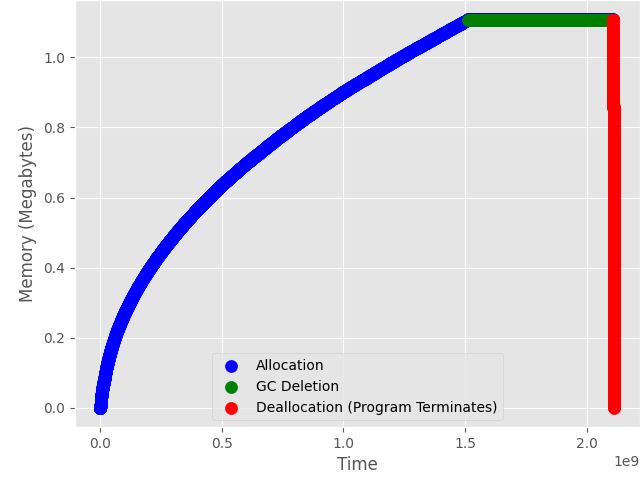
\includegraphics[width=0.47\textwidth]{marksweep_manyobjects.png}}}%
    \qquad
    \subfloat[\centering Reference Counting]{{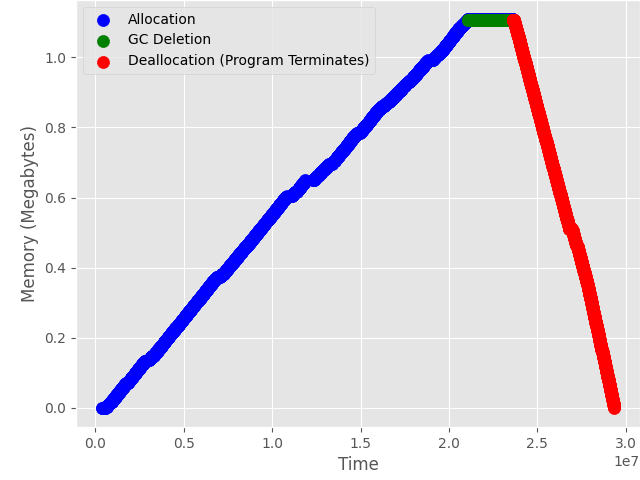
\includegraphics[width=0.47\textwidth]{refcounting_manyobjects.png} }}%
    \caption{Memory usage for large heap benchmark}
\end{figure}

Both graphs look relatively similar. However, the Reference Counting version took significantly less time to execute. The runtime of the program when using Mark Sweep was 2114.02 milliseconds, while the Reference Counting version only took 29.38 milliseconds. Reference Counting is often discarded for its slow performance, but in this scenario it managed to vastly outperformed Mark Sweep. This scenario is both the worst case for Mark Sweep, and the best for Reference Counting.

\medskip
Mark Sweep can be modified to perform better in this type of scenario, using a technique called Generational Collection. Generational collectors take advantage of the following empirical observation: the majority of objects live a very short time, while the remaining minority tends to live a very long time. 

Generational collectors segregate objects into multiple categories based on age. All objects are initially placed in a young group. Once an object has survived a number of collections cycles, it is advanced to an older group, collected less frequently than the younger group. Applying generational collection to the cycles program would prevent the Mark Sweep collector from traversing through all 1000 nodes at every single GC cycle (200 of them). Instead, the 1000 nodes would quickly be placed in an older generation, that the collector would seldom traverse. 

\subsubsection{Delayed Collection}

Reference Counting implements immediate deletion of an object as soon as it reaches a refcount of zero. This can be very useful in certain scenarios, and fail spectacularly in others. Take for example the following program: 

\begin{lstlisting}[numbers=left]
    var x = allocate 1;
    var a;
    var b;
    var c;

    for (var i = 0; i < 5000; i = i + 1){
        x = allocate 1;
        a = x;
        b = x;
        c = x;
    }

    collect;
\end{lstlisting}

This Lox program allocates 5000 memory chunk objects of \SI{1}{\kilo\byte} each on the heap. Every memory chunk contains four references to it (\lstinline{x, a, b, c}), which forces the Reference Counting collector to update the refcount of each object 8 times (from 0 to 4 and from 4 to 0). Note that just like the large heap benchmark, the variable \lstinline{x} is overwritten after every iteration. This causes the previously allocated object to become unreachable and thus garbage. However, there is no collect statement at the end of the loop's body. Instead, it is included at the end of the program. This is because we want to avoid triggering a GC cycle for Mark Sweep until after the 5000 objects are created \footnote{This is assuming the threshold for triggering a GC cycle is high enough to not be reached during the 5000 allocations. This is a reasonable assumption, since programs will often need to create many objects of a small size.}. 

\begin{figure}[h]%
    \centering
    \subfloat[\centering Mark Sweep]{{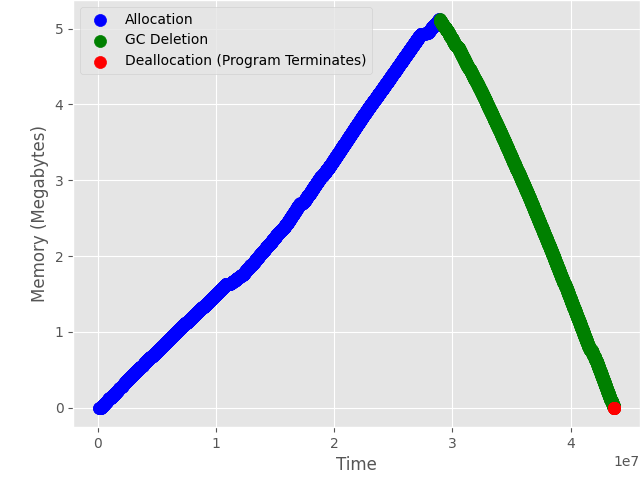
\includegraphics[width=0.47\textwidth]{marksweep_delayed.png}}}%
    \qquad
    \subfloat[\centering Reference Counting]{{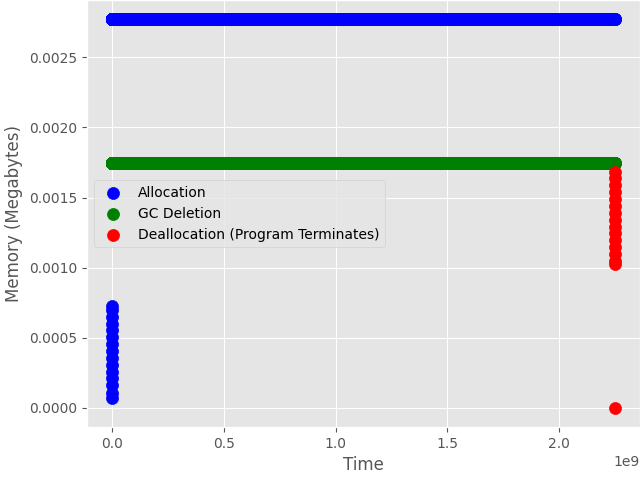
\includegraphics[width=0.47\textwidth]{refcounting_delayed.png} }}%
    \caption{Memory usage for delayed collection benchmark}
\end{figure}

The Mark Sweep graph shows how 5000 objects are created, and then all deleted in one single sweep. The Reference Counting graph shows the allocation of the memory chunk and its immediate deletion by the GC, repeated 5000 times. A closeup of the middle section of the graph shown in figure \ref{fig:refcounting_delayed_close} shows that process in more detail.

\begin{wrapfigure}{l}{0.30\textwidth}
    \vspace{-\baselineskip}
    \begin{center}
        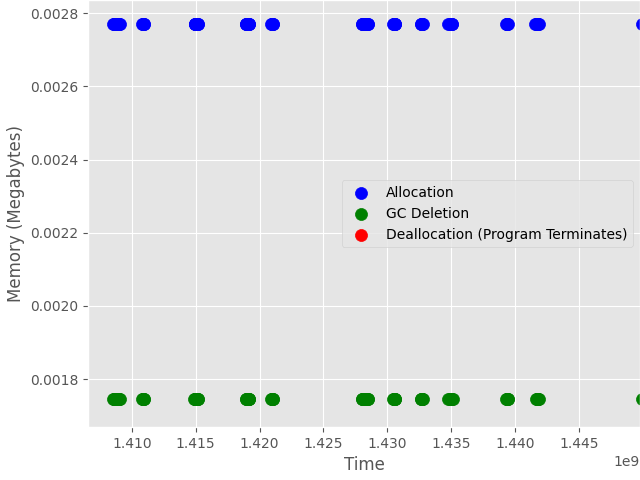
\includegraphics[width=0.29\textwidth]{refcounting_delayed_close.png}
    \end{center}
    \captionsetup{font={small}}
    \caption{Closeup of Reference Counting graph}
    \label{fig:refcounting_delayed_close}
  \end{wrapfigure}



\medskip
The big disparity between the two algorithms comes in their performance. When using Mark Sweep, the runtime of the program was 43.71 milliseconds, compared to 2248.62 milliseconds for Reference Counting. This scenario is the best case for Mark Sweep, since it only has to perform one cycle that clears all the garbage objects, achieving maximum efficiency. Conversely, this scenario is the worst case for Reference Counting 

\clearpage
\newpage 

\section{Conclusion}

Every decision made when designing a Programming language is based on tradeoffs, and garbage collection is no different. As modern programming languages move toward memory management schemes abstracted and hidden away from the programmer, it is important to understand what is happening behind the scenes, and how the performance of a program can be affected. 

This research project gave an overview of the implementation of Mark Sweep and Reference Counting, and explored the performance of those algorithms in different scenarios. Mark Sweep excels at deleting many objects at once, but requires program execution to halt completely and introduces the additional complexity of when to trigger a collection cycle. Reference Counting has the benefit of distributing GC overhead across the program through immediate collection, but frequent refcount updates are often inefficient, and cycles in memory can never be freed  . Both algorithms can be modified to perform better, through techniques such as Generational Collection and weak pointers. Furthermore, Mark Sweep and Reference Counting are often used as building blocks for more complex and domain-specific collection algorithms, such as Mark-Compact collectors, incremental/concurrent collectors, and copying collectors. When designing a programming language, the implementation of garbage collection should be carefully investigated and designed for the purpose of the language.

\subsection{Acknowledgement}

I would like to thank Professor Jonathan Shidal from the CSE department at Washington University in St. Louis for providing excellent guidance during the development of this project.

\end{document} 